% Create title frame
\titleframe

%--------------------------------------
% Table of contents
\begin{frame}{Overview}
    \setbeamertemplate{section in toc}[sections numbered]
    \tableofcontents[hideallsubsections]
\end{frame}

\begin{frame}{Credits}
Some slides are inspired by a former version of the lecture given by Jonathan Dumas.
\begin{center}
\href{https://github.com/jonathandumas/ELEN0445-1-microgrids-forecasting/blob/2b91cfc1b637b2ff17b13786b2407df66b6ac485/pdf/ELEN0445-1-microgrids-forecasting-lesson-1-2021.pdf}{\underline{Link to the GitHub page of Jonathan}}
\end{center}
\end{frame}

\section{What is a forecast}

\begin{frame}{Definition of the forecasting problem}
\begin{columns}
\begin{column}{0.45\textwidth}
We are 
\begin{itemize}
    \item at time $t$ (e.g., at 8 am, planning the operation of the microgrid)
    \item interested in what will happen at time ${t}+{k}$, $\forall k \in \{1, 2, ..., T\}$
    \begin{itemize}
        \item ${k}$ is the \textbf{lead time}
        \item $T$ is the \textbf{forecasting horizon}
    \end{itemize} 
    \item for the random variable $Y_{t+k}$, (e.g. $Y$ represents the PV production)
\end{itemize}
\end{column}
\begin{column}{0.45\textwidth}
    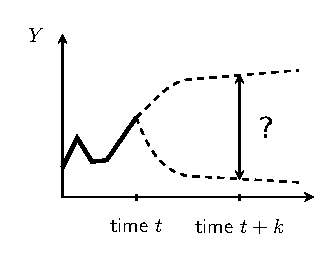
\includegraphics[width=\textwidth]{images/forecast.pdf}
\end{column}
\end{columns}

The most common way is to produce a \textbf{point forecast} (see next slide).
It is not the only way.
\end{frame}

\begin{frame}{Point Forecast}
    \begin{block}{Definition}
        A single numerical value representing the "best" estimate of the future outcome based on current information $\mathcal{F}_t$.
    \end{block}

    \vspace{0.5cm}
    Usually expressed as the \textbf{conditional expectation}:
    $$\hat{y}_{t+k|t} = E[Y_{t+k} | \mathcal{F}_t]$$

    \begin{itemize}
        \item \textbf{Goal:} Minimize a symmetric loss function (like Mean Squared Error).
        \item \textbf{Output:} A single scalar.
    \end{itemize}
\end{frame}


\begin{frame}{Density Forecast}
    \begin{block}{Definition}
        An estimate of the entire probability distribution of the random variable at time $t+k$.
    \end{block}

    \vspace{0.5cm}
    Expressed as the \textbf{conditional density function}:
    $$f(y_{t+k} | \mathcal{F}_t)$$

    \begin{itemize}
        \item \textbf{Goal:} Provide a complete description of uncertainty.
        \item \textbf{Output:} A function (e.g., a Normal distribution $\mathcal{N}(\mu, \sigma^2)$).
    \end{itemize}
\end{frame}


\begin{frame}{Quantile Forecast}
    \begin{block}{Definition}
        The value $q$ such that there is a probability $\alpha$ of the realization falling below it.
    \end{block}

    \vspace{0.3cm}
    Formally defined as:
    $$Q_{\alpha}(Y_{t+k} | \mathcal{F}_t) = \inf \{ y : P(Y_{t+k} \le y | \mathcal{F}_t) \ge \alpha \}$$

    In general, we forecast several quantiles.

    \textbf{Key Levels:}
    \begin{itemize}
        \item $\alpha = 0.5$: the \textbf{median} forecast.
        \item $\alpha = 0.05 / 0.95$: the \textbf{Value at Risk }(VaR) or tail-risk boundaries.
    \end{itemize}

    

\end{frame}

\begin{frame}{Underlying assumption: piecewise constant forecast ($\Delta t$)}
\begin{columns}
\begin{column}{0.4\textwidth}
\begin{itemize}
    \item A time step $t$ has a duration $\Delta t$ (e.g. 15 min)
    \item The forecasted quantity is assumed constant over this period, i.e. we are forecasting only one value (or one distribution or one set of quantiles)
\end{itemize}
\end{column}
\begin{column}{0.55\textwidth}
    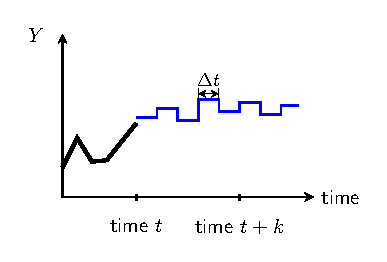
\includegraphics[width=\textwidth]{images/forecast_quantized.pdf}
\end{column}
\end{columns}
\end{frame}

\begin{frame}{Convention: Zero-Order Hold (ZOH)}
\begin{columns}
    \begin{column}{0.45\textwidth}
        \includegraphics[width=\textwidth]{images/ZOH.pdf}
    \end{column}

    \begin{column}{0.555\textwidth}
        \begin{itemize}
            \item The value at the start of the interval persists until the next update.
            \item Mathematically: 
            $$Y(\tau) = \hat{y}(t), \ \forall \tau \in [t, t + \Delta t) $$
            \item Creates the characteristic \textbf{staircase} profile.
        \end{itemize}
    \end{column}
\end{columns}
Example: 
\begin{itemize}
    \item if time step $t$ corresponds to time 08:00, 
    \item we will assume that the forecast is constant from $t$ to $t+\Delta t$ (e.g. 8:00 to 8:15).
\end{itemize}
\end{frame}

\begin{frame}[allowframebreaks]{PV generation forecasting example}
PV point forecasts (dad 24) are computed using a neural network at noon
for the next day, and the corresponding observations are in red (Pm).
\begin{center}
    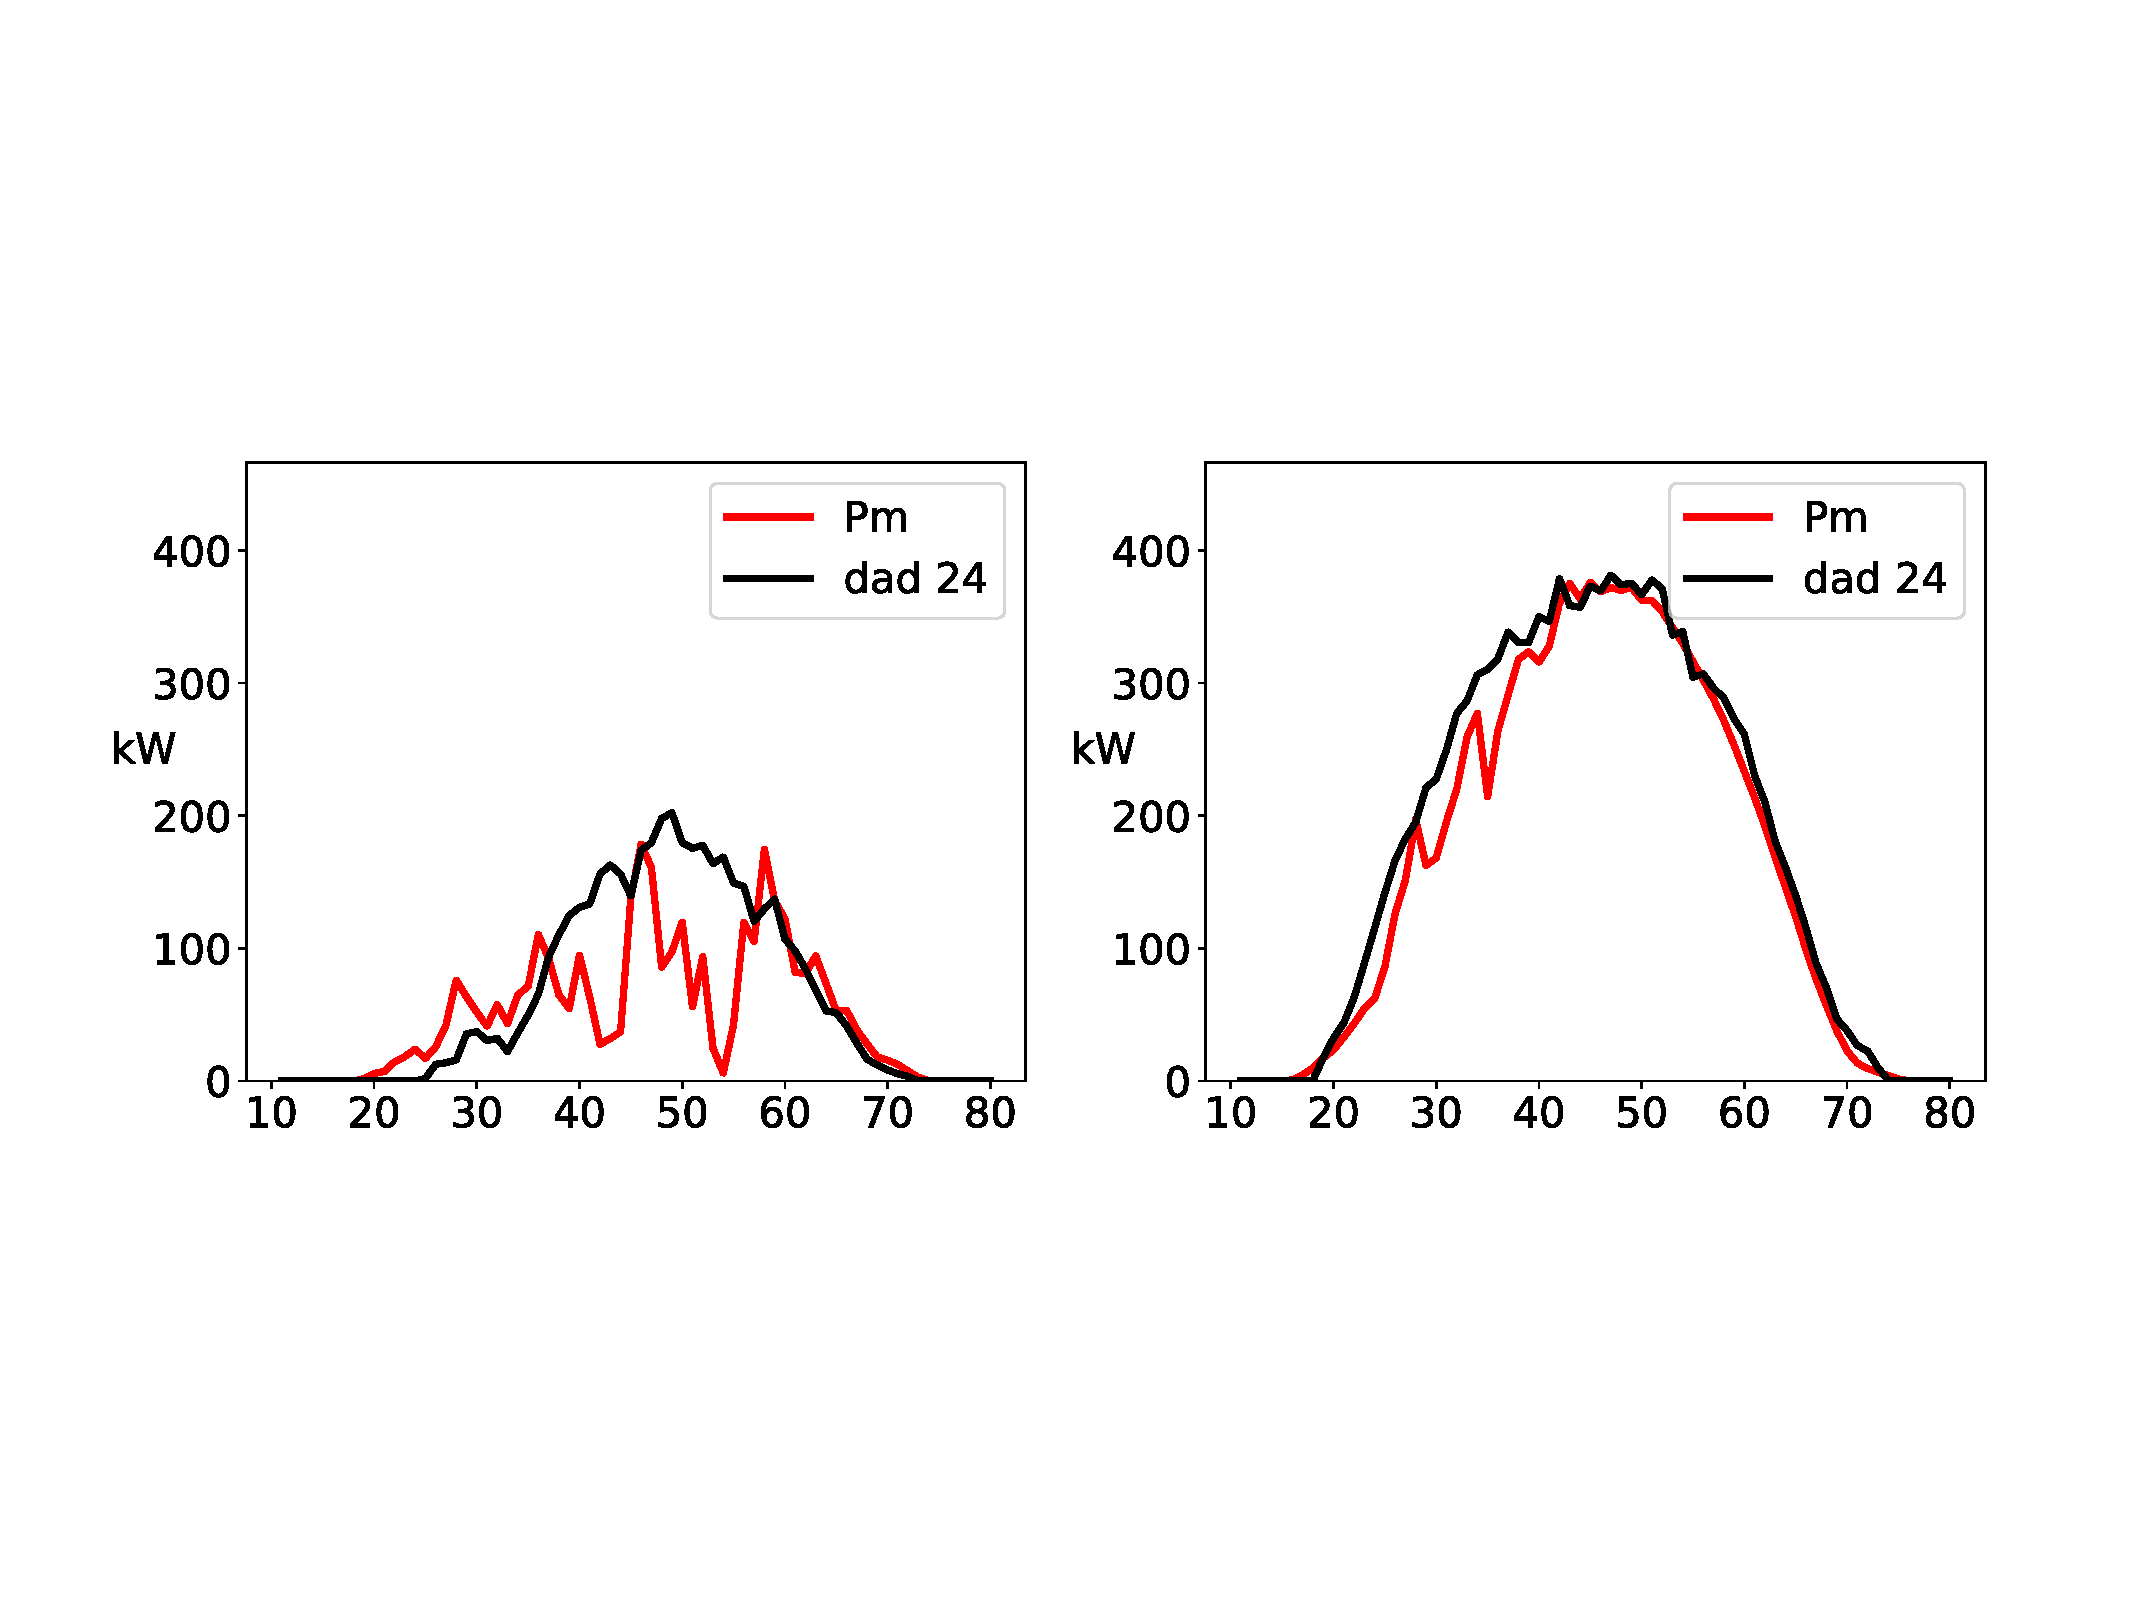
\includegraphics[width=0.7\textwidth]{images/PV_forecast_example.pdf} \\
\end{center}


Inputs to the neural network: numerical weather forecasts of 
\begin{itemize}
    \item solar irradiation 
    \item air temperature.
\end{itemize}


\textit{
Reference: \\
J. Dumas, C. Cointe, X. Fettweis and B. Cornélusse, "Deep learning-based multi-output
quantile forecasting of PV generation," 2021 IEEE Madrid PowerTech, 2021, pp. 1-6, doi:
10.1109/PowerTech46648.2021.9494976.}
\end{frame}


% Section: The Value of Forecasting
\section{Why forecasting? A decision-making perspective}

% Slide: Operational Planning
\begin{frame}{Operational planning: the 24h–48h horizon}
    \begin{itemize}
        \item \textbf{Unit Commitment:} Deciding which local generators (e.g., Diesel GenSets, CHP) to turn ON/OFF to minimize startup costs / degradation.
        \item \textbf{Battery Energy Storage (BESS) Dispatch:} 
        \begin{itemize}
            \item Should we charge now from the grid (low price) or wait for the solar peak (free)?
            \item Requires accurate $P_{net} = P_{load} - P_{gen}$ forecasts.
        \end{itemize}
        \item \textbf{Demand Response (DR):} Scheduling shiftable loads (HVAC, EV charging) to align with renewable availability.
    \end{itemize}
    \begin{block}{The "Cost" of Uncertainty}
        \begin{itemize}
            \item Under-forecasting solar might lead to unexpected grid peak charges
            \item over-forecasting might lead to a depleted battery when it's needed most.
        \end{itemize}
    \end{block}
\end{frame}

% Slide: Long-Term Sizing
\begin{frame}{Sizing \& Investment: the multi-year horizon}
    Long-term forecasts (10–20 years) drive the \textbf{Optimal Sizing} of assets.
    \vspace{0.2cm}
    \begin{itemize}
        \item \textbf{Capital Expenditure (CAPEX):} If we over-forecast load growth, we over-invest in generation devices and batteries that remain underutilized.
        \item \textbf{Reliability Targets:} Using "Typical Meteorological Year" (TMY) data to ensure the microgrid can survive a 3-day "dunkelflaute" (no sun/wind).
        \item \textbf{Degradation Modeling:} Forecasting long-term usage patterns to predict when the BESS or fuel cell will need replacement.
    \end{itemize}
    \vspace{0.2cm}
    \textbf{Caution:} when forecasting/deciding for long term, care about the \alert{time value of money}!
\end{frame}

% Slide: Grid-Connected Forecasting
\begin{frame}{Grid-connected: economic optimization}
    In this mode, the utility grid acts as an "infinite battery" or a safety net.
    \begin{itemize}
        \item \textbf{Objective:} Profit Maximization / Bill Reduction.
        \item \textbf{Forecast Impact:} 
        \begin{itemize}
            \item Errors lead to \textbf{sub-optimal trading} (e.g., buying power at peak prices).
            \item Deviation from "Day-Ahead" commitments may result in \textbf{imbalance penalties} from the utility (only for large microgrids for those who have to do these commitments)
        \end{itemize}
        \item \textbf{Safety Margin:} Low. The grid absorbs your volatility.
    \end{itemize}
    \begin{exampleblock}{Key Metric}
        Focus on \textbf{MAPE} and \textbf{Daily Operational Cost}. A 10\% error might cost \$500 in lost savings, but the lights stay on.
    \end{exampleblock}
\end{frame}

% Slide: Islanded Forecasting
\begin{frame}{Islanded mode: surviving}
    Whether in a remote area or because of a grid outage, no safety net.
    \begin{itemize}
        \item \textbf{Objective:} System stability and load shedding minimization.
        \item \textbf{Forecast Impact:}
        \begin{itemize}
            \item \textbf{Under-forecasting Load:} Can lead to a sudden frequency drop and a total system blackout.
            \item \textbf{Over-forecasting Solar:} May cause the battery to hit "Zero State of Charge" (0\% SoC) at 2 AM.
        \end{itemize}
        \item \textbf{Safety Margin:} High. You must use \textbf{Probabilistic Quantiles} (e.g., $q_{0.95}$) to ensure reserves are always available.
    \end{itemize}
    \begin{alertblock}{Critical Change}
        In Islanded mode, we care more about the \textbf{Lower Bound} of generation and the \textbf{Upper Bound} of load to guarantee "Survivability."
    \end{alertblock}
\end{frame}

% Slide: Comparison Table
\begin{frame}{Summary: Accuracy vs. Resilience}
    \begin{table}
        \centering
        \small
        \begin{tabular}{lll}
            \toprule
            Feature & \textbf{Grid-Connected} & \textbf{Islanded (Off-Grid)} \\
            \midrule
            \textbf{Primary Goal} & Economic Optimization & System Reliability \\
            \textbf{Error Result} & Financial Loss & Blackout / Load Shedding \\
            \textbf{Forecast Type} & Point (Deterministic) & Probabilistic (Uncertainty) \\
            \textbf{Risk Appetite} & Moderate & Zero to Very Low \\
            \textbf{Key Resource} & Market Price Signal & Battery State of Charge \\
            \bottomrule
        \end{tabular}
    \end{table}
\end{frame}


% Section 2: Deterministic ML
\section{Deterministic point forecasts}
\begin{frame}{Procedure}
\begin{tikzpicture}[
    % Define the style for the boxes
    block/.style={
        rectangle, 
        draw,  
        text width=7em, 
        text centered, 
        rounded corners, 
        minimum height=5em
    },
    % Define the style for the arrows
    line/.style={
        draw, 
        -Latex, 
        thick
    }
]

    % Place the nodes (boxes)
    \node [block] (box1) {Select Data};
    \node [block, right=1cm of box1] (box2) {Select Forecasting methods};
    \node [block, right=1cm of box2] (box3) {Run experimental protocol and fit model};
    \node [block, right=1cm of box3] (box4) {Deploy};

    % Draw the arrows
    \path [line] (box1) -- (box2);
    \path [line] (box2) -- (box3);
    \path [line] (box3) -- (box4);

\end{tikzpicture}
\end{frame}


\begin{frame}{Procedure}
\begin{tikzpicture}[
    % Define the style for the boxes
    block/.style={
        rectangle, 
        draw, 
        text width=7em, 
        text centered, 
        rounded corners, 
        minimum height=5em
    },
    % Define the style for the arrows
    line/.style={
        draw, 
        -Latex, 
        thick
    }
]
    % Place the nodes (boxes)
    \node [block, fill=orange!20] (box1) {Select Data};
    \node [block, right=1cm of box1] (box2) {Select Forecasting methods};
    \node [block, right=1cm of box2] (box3) {Run experimental protocol and fit model};
    \node [block, right=1cm of box3] (box4) {Deploy};

    % Draw the arrows
    \path [line] (box1) -- (box2);
    \path [line] (box2) -- (box3);
    \path [line] (box3) -- (box4);

\end{tikzpicture}
\end{frame}


\subsection{Data selection and collection}
\begin{frame}{Data selection and collection}
        \begin{itemize}
            \item Which data is useful for your problem?
            \item Which data will be avaialble when using your model? Fewer dependencies, more robustness
            \item Check the integrity of the data (min-max values), time-zone, averaging convention
            \item Fill the holes in the data and/or ensure you training procedure will not be impacted 
        \end{itemize}
\end{frame}

\begin{frame}{Typical forecasting inputs}
    \begin{itemize}
    \item \textbf{Weather} variables \alert{WARNING: depends on the forecasting problem!}
        \begin{itemize}
            \item Time series: temperature, solar irradiation, wind speed, rainfall (short term)
            \item Mean/standard deviation: temperature, solar irradiation (long term)
        \end{itemize}
    \item \textbf{Calendar} variables
    \begin{itemize}
        \item days, hours of the days, special day  (short term)
        \item trend, years, months (long term)
    \end{itemize}
    \item \textbf{Historic} values
    \begin{itemize}
        \item at $t-15$ min, $t-1$ h, $t-24$ h, $t-7$ d, mean($t-1$ d) (short term)
        \item Mean/standard deviation: $t-1$ week, $t-1$ month (long term)
    \end{itemize}
    \item \textbf{Feature engineering}
    \begin{itemize}
        \item temperature $\times$ calendar variables
        \item lagged load $\times$ temperature
    \end{itemize}
    \end{itemize}
\end{frame}

\subsection{Forecasting methods}
\begin{frame}{Procedure}
    
\begin{tikzpicture}[
    % Define the style for the boxes
    block/.style={
        rectangle, 
        draw, 
        text width=7em, 
        text centered, 
        rounded corners, 
        minimum height=5em
        },
        % Define the style for the arrows
        line/.style={
            draw, 
            -Latex, 
            thick
            }
            ]
            % Place the nodes (boxes)
            \node [block] (box1) {Select Data};
            \node [block, right=1cm of box1, fill=orange!20] (box2) {Select Forecasting methods};
            \node [block, right=1cm of box2] (box3) {Run experimental protocol and fit model};
            \node [block, right=1cm of box3] (box4) {Deploy};
            
            % Draw the arrows
            \path [line] (box1) -- (box2);
            \path [line] (box2) -- (box3);
            \path [line] (box3) -- (box4);
            
        \end{tikzpicture}
    \end{frame}
\begin{frame}{Select one or more forecasting methods}
    \begin{itemize}
        \item Does a simple method yield good results? 
        \item Do you have a lot of data? 
        \item What is the nature of data?
    \end{itemize} 
\end{frame}
         
\begin{frame}{Baseline model - Persistence model}
    \begin{itemize}
        \item \textbf{Objective:} Establishing the "Minimum Viable Forecast."
        \item \textbf{Persistence Model:} The $Naive$ approach:
        \[ \hat{y}_{t+k} = y_t \]
    \end{itemize}
    \begin{exampleblock}{Pro-Tip}
        If your ML model cannot beat the Persistence Model, your features are likely poorly engineered.
    \end{exampleblock}
\end{frame}
\begin{frame}{Machine learning models}
    We move from simple averages to capturing non-linear patterns:
    \vspace{0.3cm}
    \begin{description}
        \item[Tree-Based] \textbf{XGBoost / LightGBM}: Excellent for tabular data and handling missing weather values.
        \item[Deep Learning] \textbf{LSTMs}: Captures the "memory" of power ramps in wind and solar.
    \end{description}
\end{frame}

\begin{frame}[allowframebreaks]{Multi-step Forecasting Strategies}
    To predict a horizon $T$, we must choose how to handle the lead time $k$.

    \vspace{1cm}
    
    \begin{columns}[T]
        \begin{column}{0.45\textwidth}
            \textbf{1. Recursive (Iterated)}
            \begin{itemize}
                \item A single model predicts $t+1$.
                \item The prediction $\hat{y}_{t+1}$ is fed back as an input for $t+2$.
                \item \textcolor{red}{Risk:} Error accumulation over long horizons.
            \end{itemize}
        \end{column}
        \begin{column}{0.45\textwidth}
            \textbf{2. Direct (Multi-output)}
            \begin{itemize}
                \item $T$ different models (or one multi-output NN ) predict each step independently.
                \item No error propagation.
                \item \textcolor{red}{Risk:} Ignores temporal dependencies between outputs.
            \end{itemize}
        \end{column}
    \end{columns}

    \vspace{0.8cm}

    \begin{center}
        \begin{tikzpicture}[node distance=1.5cm, every node/.style={draw, thick, fill=blue!10, minimum width=1.2cm}]
            % Recursive Diagram
            \node (in1) [rectangle] {Input $y_t$};
            \node (m1) [ellipse, right=of in1, fill=green!10] {Model};
            \node (out1) [rectangle, right=of m1] {$\hat{y}_{t+1}$};
            \draw [-Stealth] (in1) -- (m1);
            \draw [-Stealth] (m1) -- (out1);
            \draw [-Stealth, bend left=45] (out1.south) to node[draw=none, fill=none, above] {feedback} (in1.south);
            \node[draw=none, fill=none, above=0.1cm of m1] {\small \textbf{Recursive}};
            
            % Direct Diagram
            \node (in2) [rectangle, below=3cm of in1] {Input $y_t$};
            \node (m2) [ellipse, right=of in2, fill=orange!10, minimum height=1cm] {Model(s)};
            \node (out2) [rectangle, right=of m2, yshift=0.3cm] {$\hat{y}_{t+1}$};
            \node (out3) [rectangle, right=of m2, yshift=-0.3cm] {$\hat{y}_{t+k}$};
            \draw [-Stealth] (in2) -- (m2);
            \draw [-Stealth] (m2.east) -- (out2.west);
            \draw [-Stealth] (m2.east) -- (out3.west);
            \node[draw=none, fill=none, above=0.1cm of m2] {\small \textbf{Direct}};
        \end{tikzpicture}
    \end{center}
\end{frame}

\begin{frame}{Procedure}    
\begin{tikzpicture}[
    % Define the style for the boxes
    block/.style={
        rectangle, 
        draw, 
        text width=7em, 
        text centered, 
        rounded corners, 
        minimum height=5em
        },
        % Define the style for the arrows
        line/.style={
            draw, 
            -Latex, 
            thick
            }
            ]
            % Place the nodes (boxes)
            \node [block] (box1) {Select Data};
            \node [block, right=1cm of box1] (box2) {Select Forecasting methods};
            \node [block, right=1cm of box2, fill=orange!20] (box3) {Run experimental protocol and fit model};
            \node [block, right=1cm of box3] (box4) {Deploy};
            
            % Draw the arrows
            \path [line] (box1) -- (box2);
            \path [line] (box2) -- (box3);
            \path [line] (box3) -- (box4);
            
\end{tikzpicture}
\end{frame}

% Slide: Time-Series Cross Validation
\begin{frame}{Define an experimental protocol to train and test your Models and \textbf{Avoid Data Leakage}}
    \textbf{Time order is important}! Shuffling your data for Cross-Validation (CV) is a critical error.
    \vspace{0.3cm}
    \begin{itemize}
        \item \textbf{Data Leakage:} If the model sees tomorrow's weather to predict today's load, its accuracy is an illusion.
        \item \textbf{Forward Chaining CV:}
        \begin{itemize}
            \item Fold 1: Train [Jan], Validate [Feb]
            \item Fold 2: Train [Jan-Feb], Validate [Mar]
            \item Fold 3: Train [Jan-Mar], Validate [Apr]
        \end{itemize}
    \end{itemize}
    \begin{block}{The Test Set}
        Always keep the final 10–15\% of your most recent data (e.g., the last 3 months) completely untouched until the very end.
    \end{block}
\end{frame}

% Slide: Combatting Overfitting
\begin{frame}{Avoiding Overfitting in Energy Models}
    How to ensure the model generalizes to new weather patterns:
    \vspace{0.2cm}
    \begin{enumerate}
        \item \textbf{Feature Selection:} Don't throw 100 weather variables at the model. Use \textit{Correlation Heatmaps} to pick the most impactful ones.
        \item \textbf{Early Stopping:} Stop training when the \textbf{Validation Loss} starts to rise, even if Training Loss is still falling.
        \item \textbf{Hyperparameter Tuning:} Use a "Grid Search" or "Bayesian Optimization" specifically within the Time-Series Split framework (e.g. \href{https://optuna.org/}{\alert{\underline{Optuna}}})
    \end{enumerate}
    \vspace{0.2cm}
    \textbf{Result:} A model that learns the \textit{physics} of the microgrid, not the \textit{noise} of the sensors.
\end{frame}

\subsection{Error sources}

\begin{frame}{Numerical weather forecast errors}

Weather forecasts errors most often drive the forecasting errors.
Typical errors are amplitude errors (left below) and phase errors (right
below).

\begin{center}
    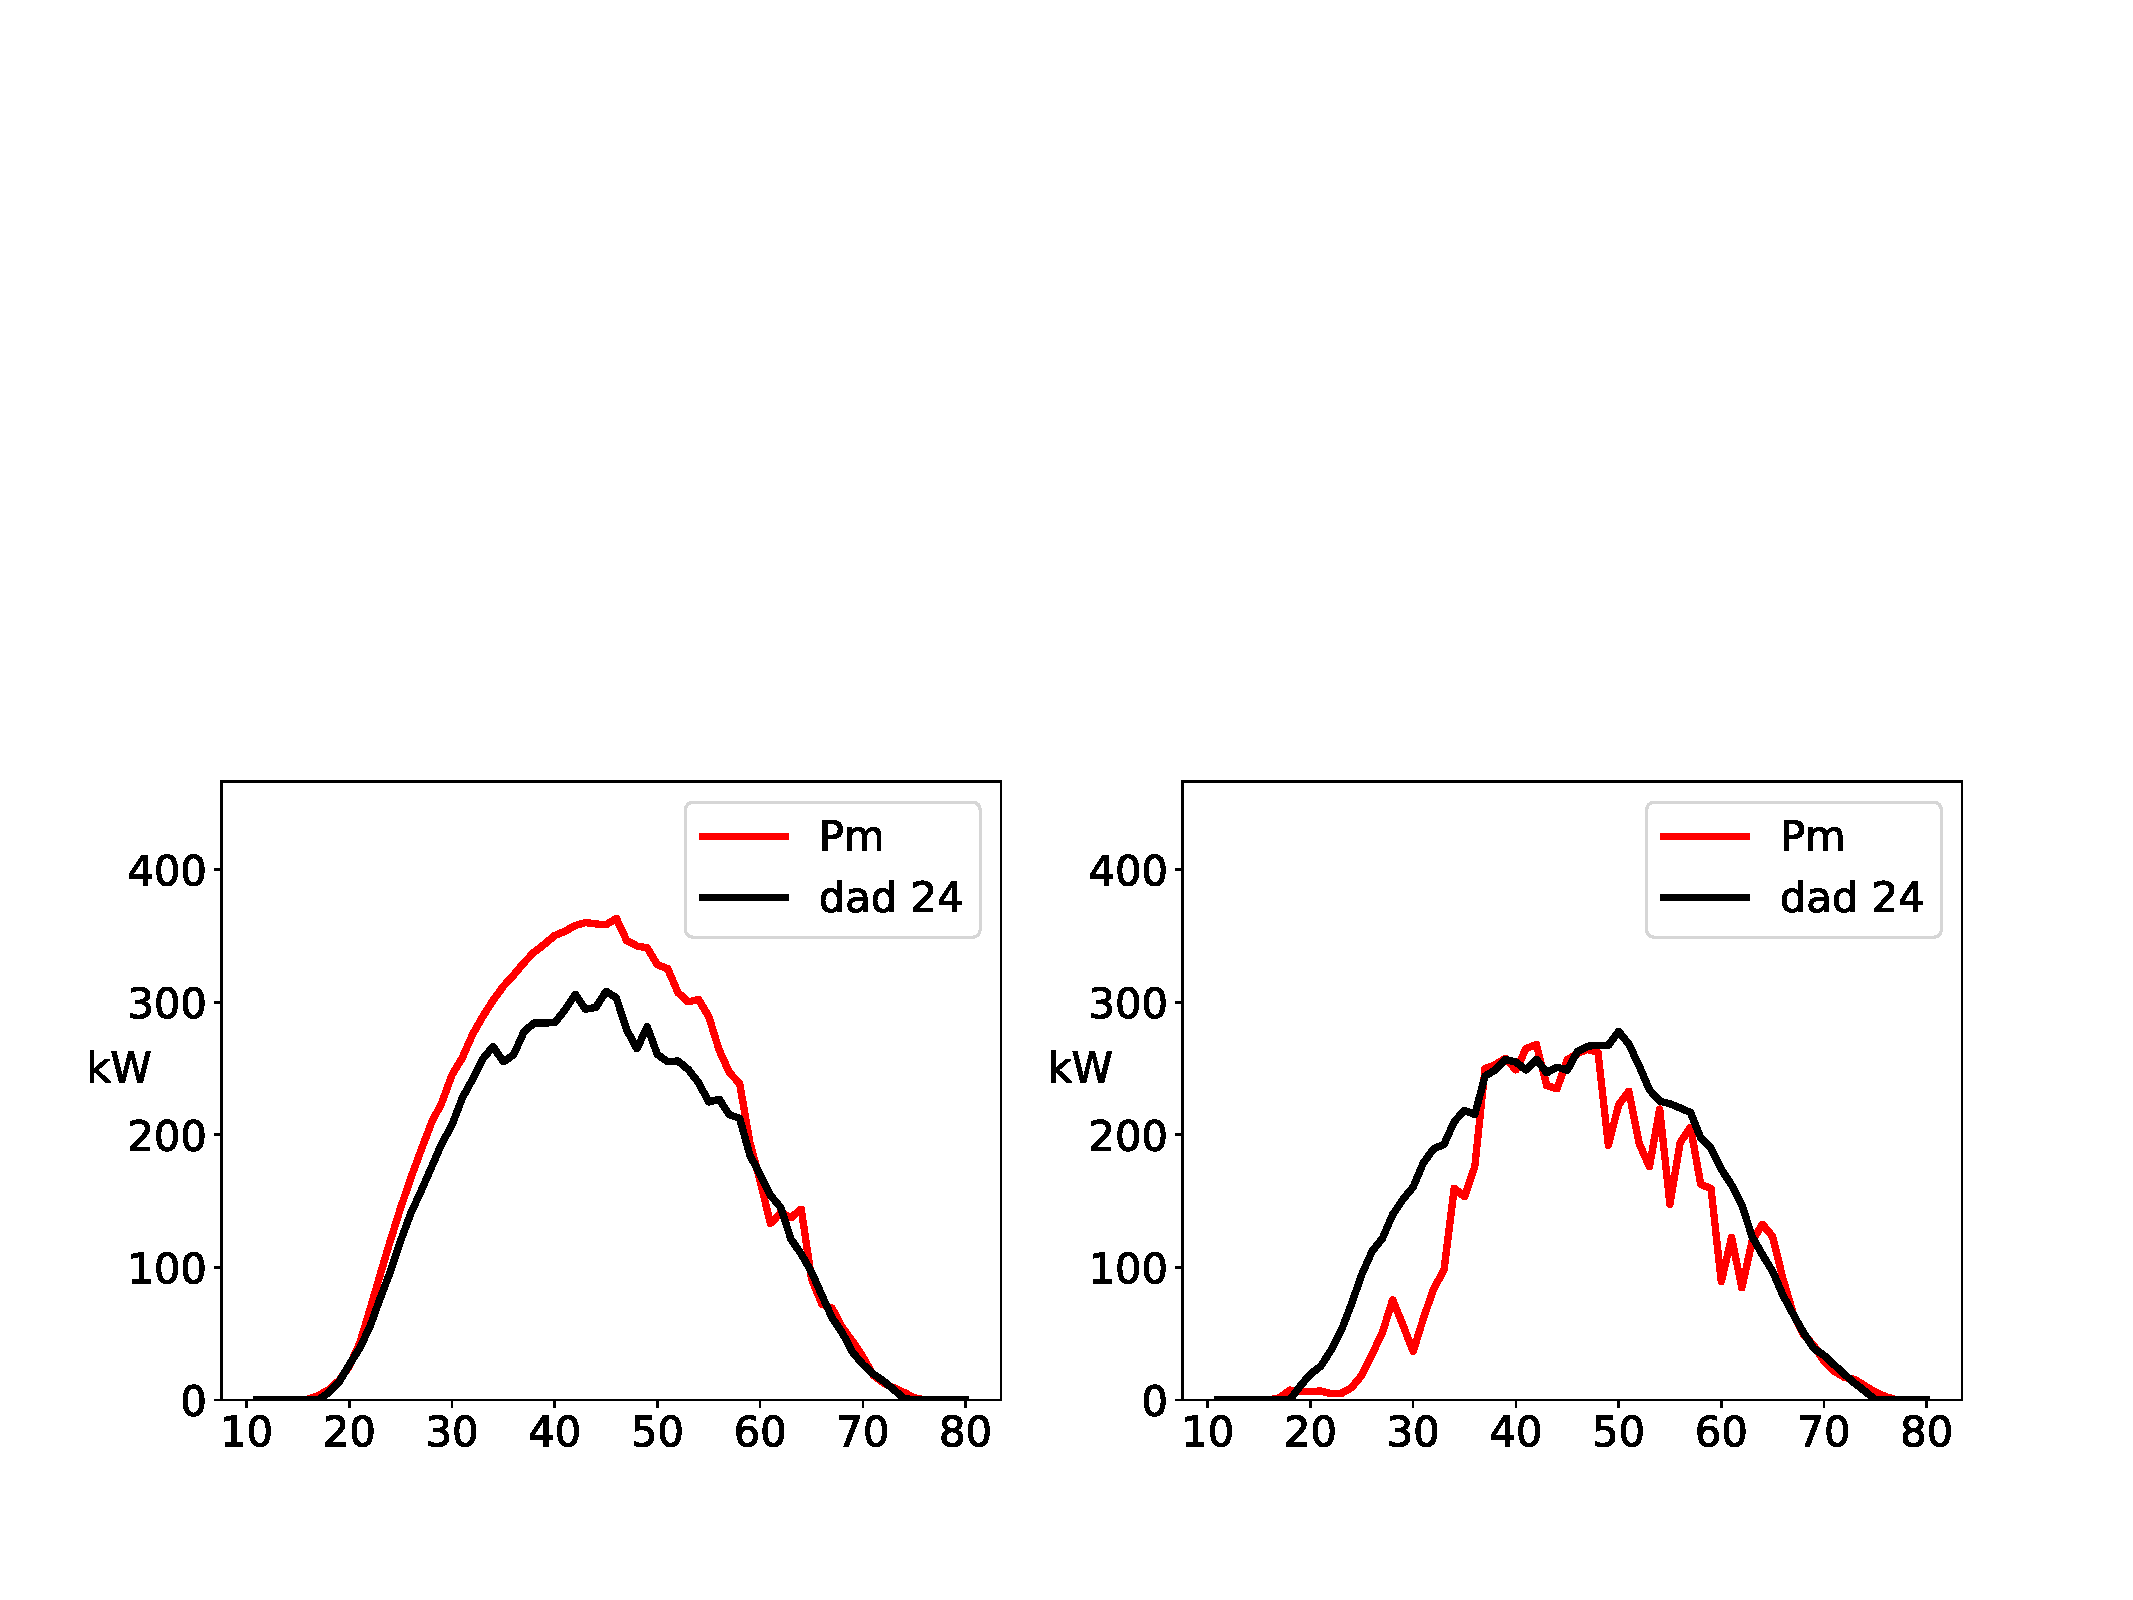
\includegraphics[width=0.8\textwidth]{images/amplitude_phase_errors.pdf}    
\end{center}

\end{frame}


\subsection{Evaluating Performance}

\begin{frame}{Visual inspection}

Visual inspection offers significant insight into forecast trends. 
While it remains a strictly a qualitative assessment, it is key in the development process.

\textit{What do you think of these two? Are they good or bad?
}\begin{columns}
  \begin{column}{0.45\textwidth}
    \begin{center}
        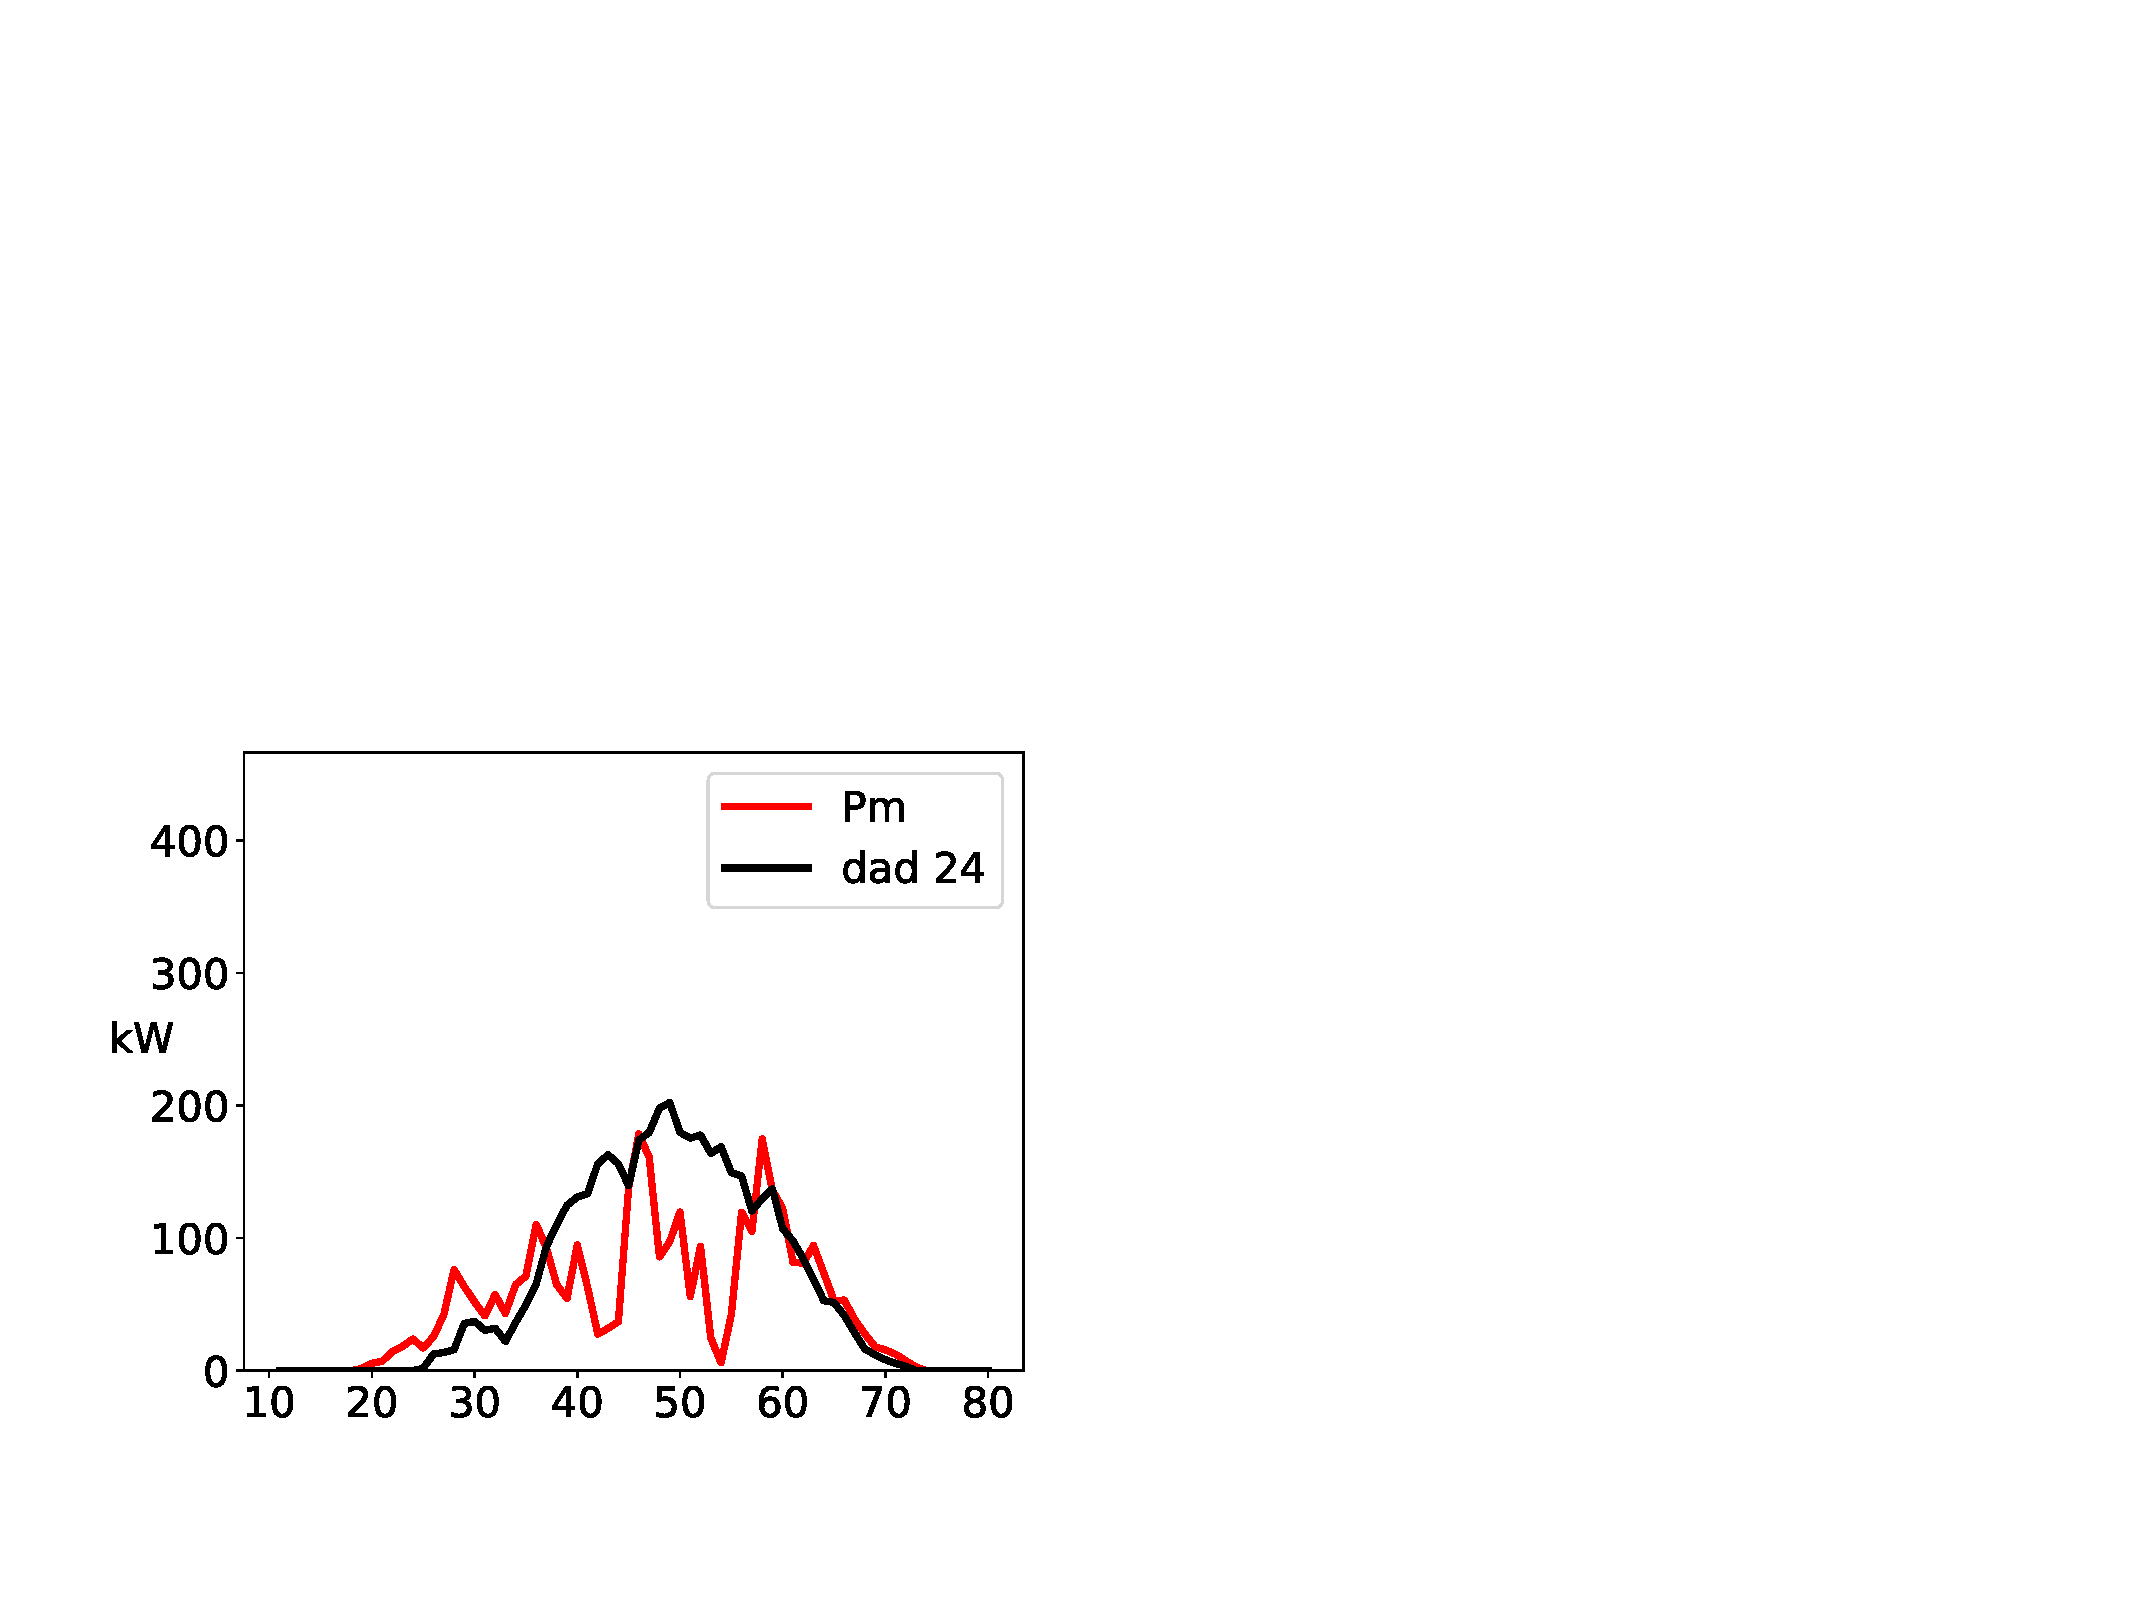
\includegraphics[width=0.7\textwidth]{images/PV_april_3_2020.pdf}\\
        {\small \it Issued on April 3, 2020 at 12:00 for April 4, 2020.}
    \end{center}
  \end{column}
  \begin{column}{0.45\textwidth}
    \begin{center}
        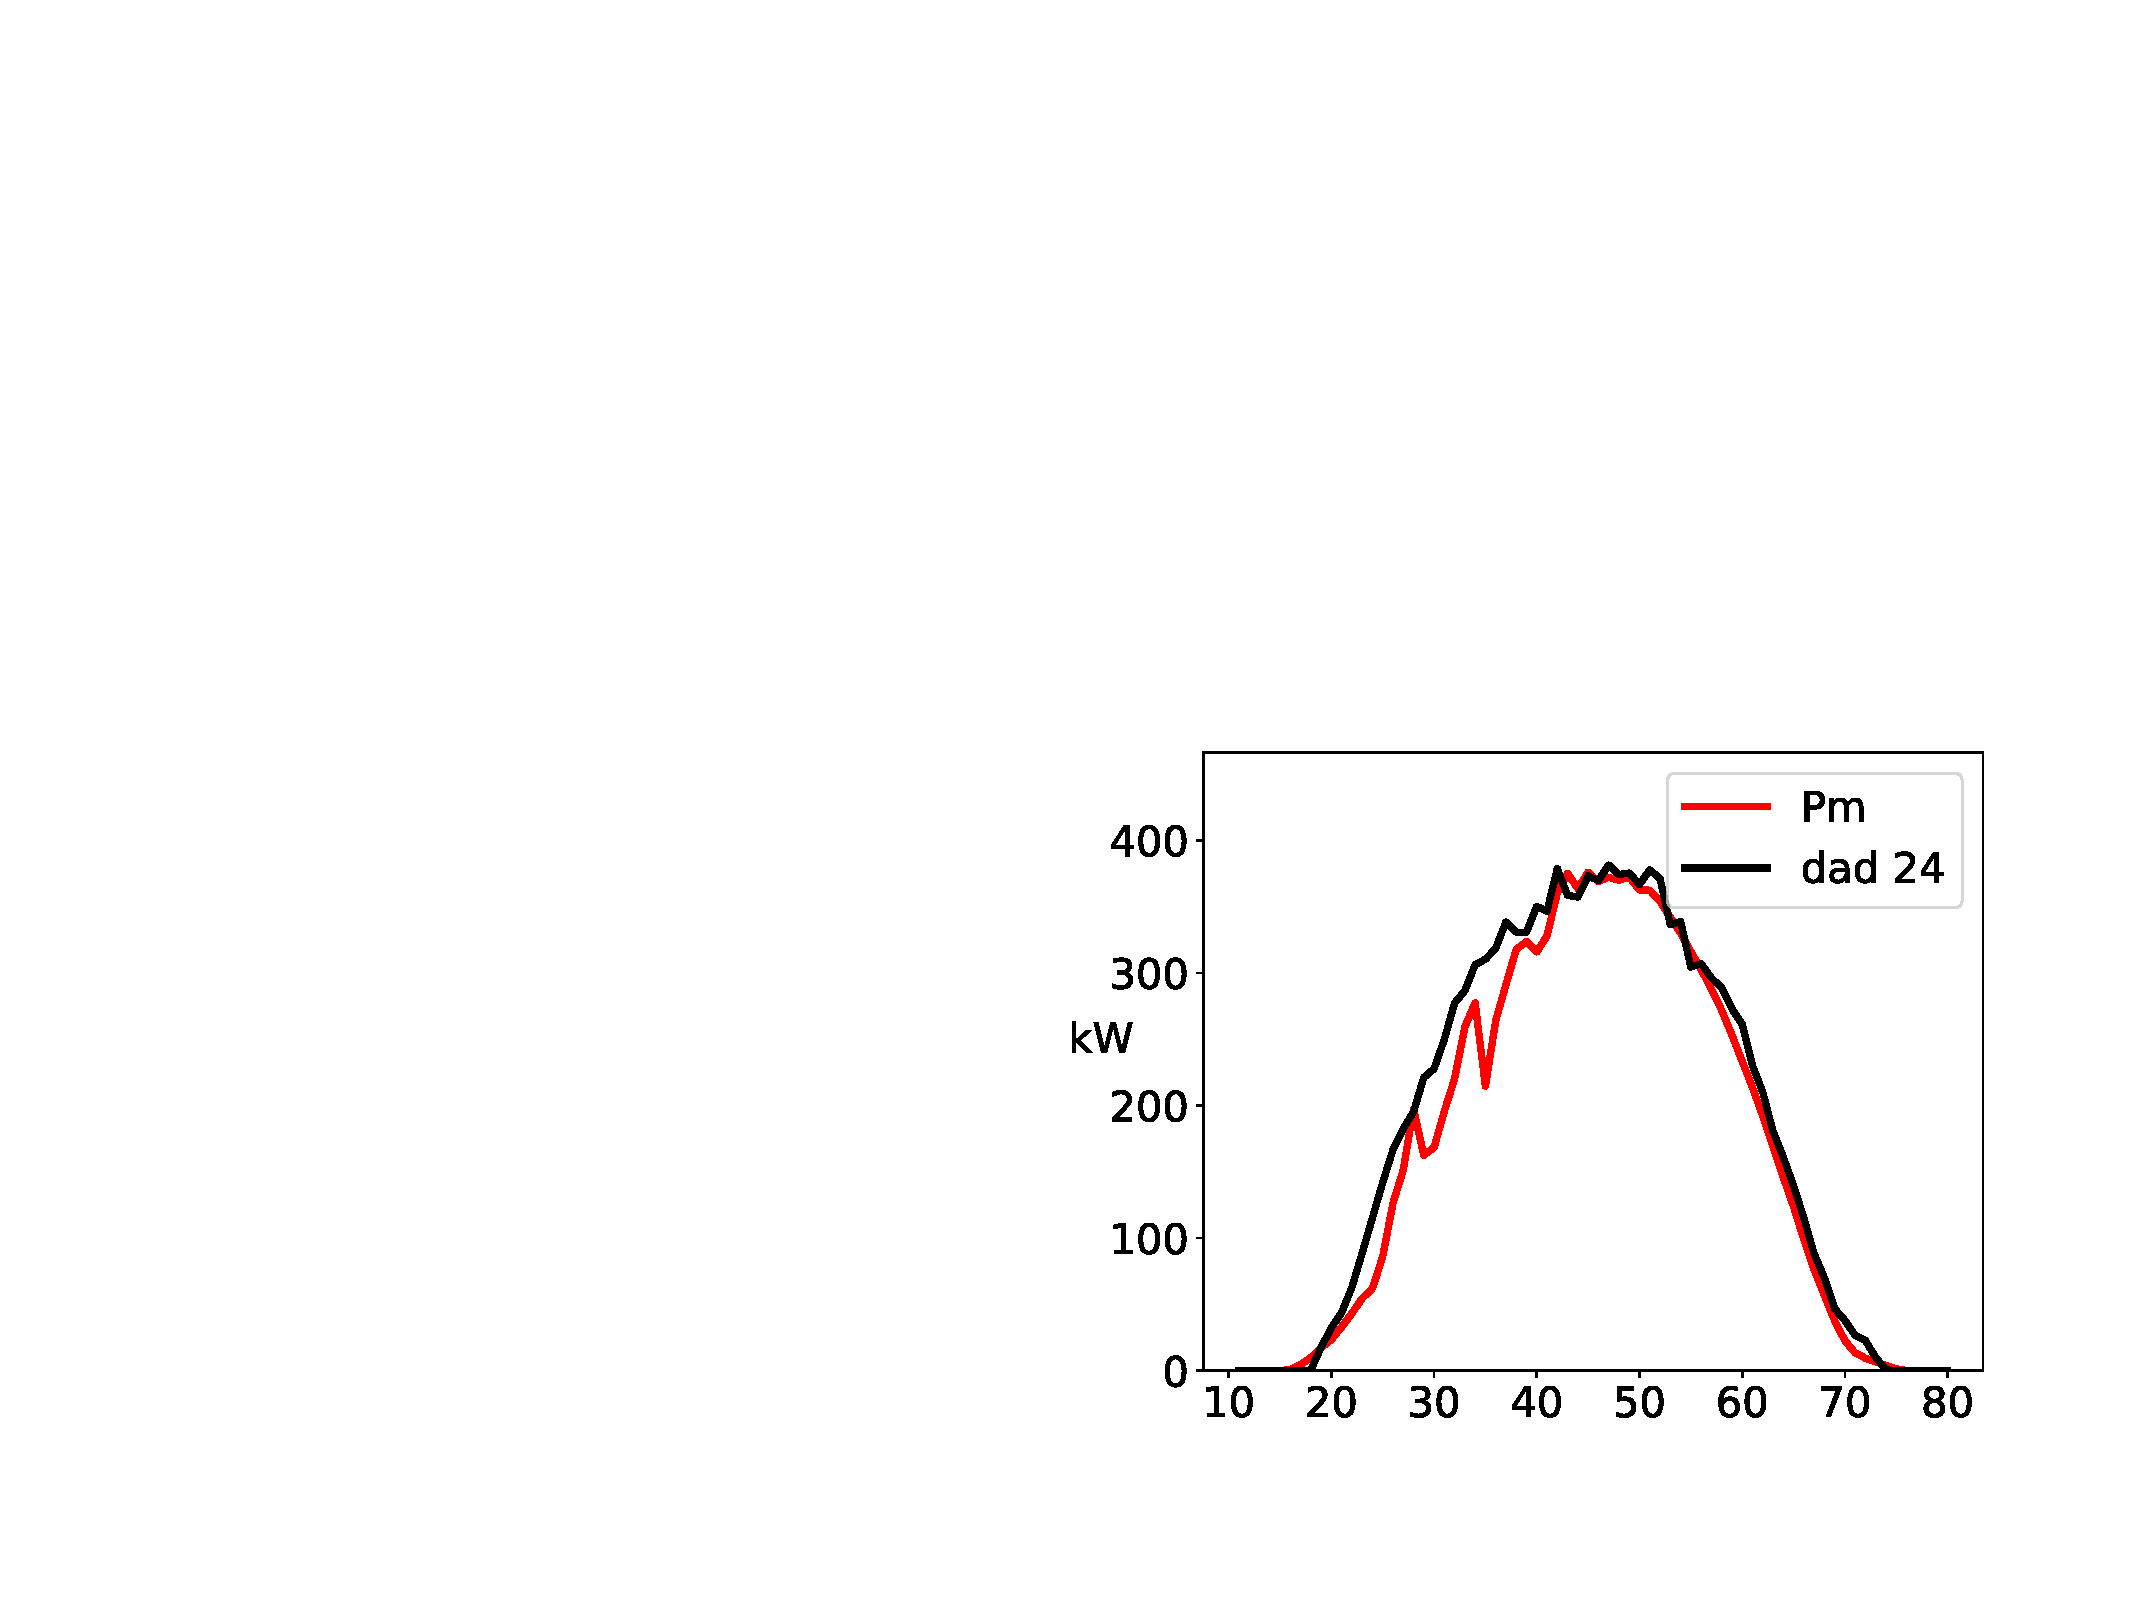
\includegraphics[width=0.7\textwidth]{images/PV_may_4_2020.pdf}\\
        {\small \it Issued on May 4, 2020 at 12:00 for May 5, 2020.}
    \end{center}
  \end{column}
\end{columns}
\end{frame}

\begin{frame}{Qualitative analysis ought to be complemented by quantitative analysis.}


Let $y$ be a realization and $\hat{y}$ a forecast.

The \textbf{forecast error} is defined by
$$
\varepsilon_{t+k \mid t}=y_{t+k \mid t}-\hat{y}_{t+k \mid t}
$$

It can be \textbf{normalized}
$$
\bar{\varepsilon}_{t+k \mid t}=\frac{y_{t+k \mid t}-\hat{y}_{t+k \mid t}}{P_n}
$$
with $P_n$ the nominal capacity (assuming a plant can generate a power between $0$ and $P_n$).

\end{frame}

\begin{frame}{Illustration of forecast error: a wind farm}
    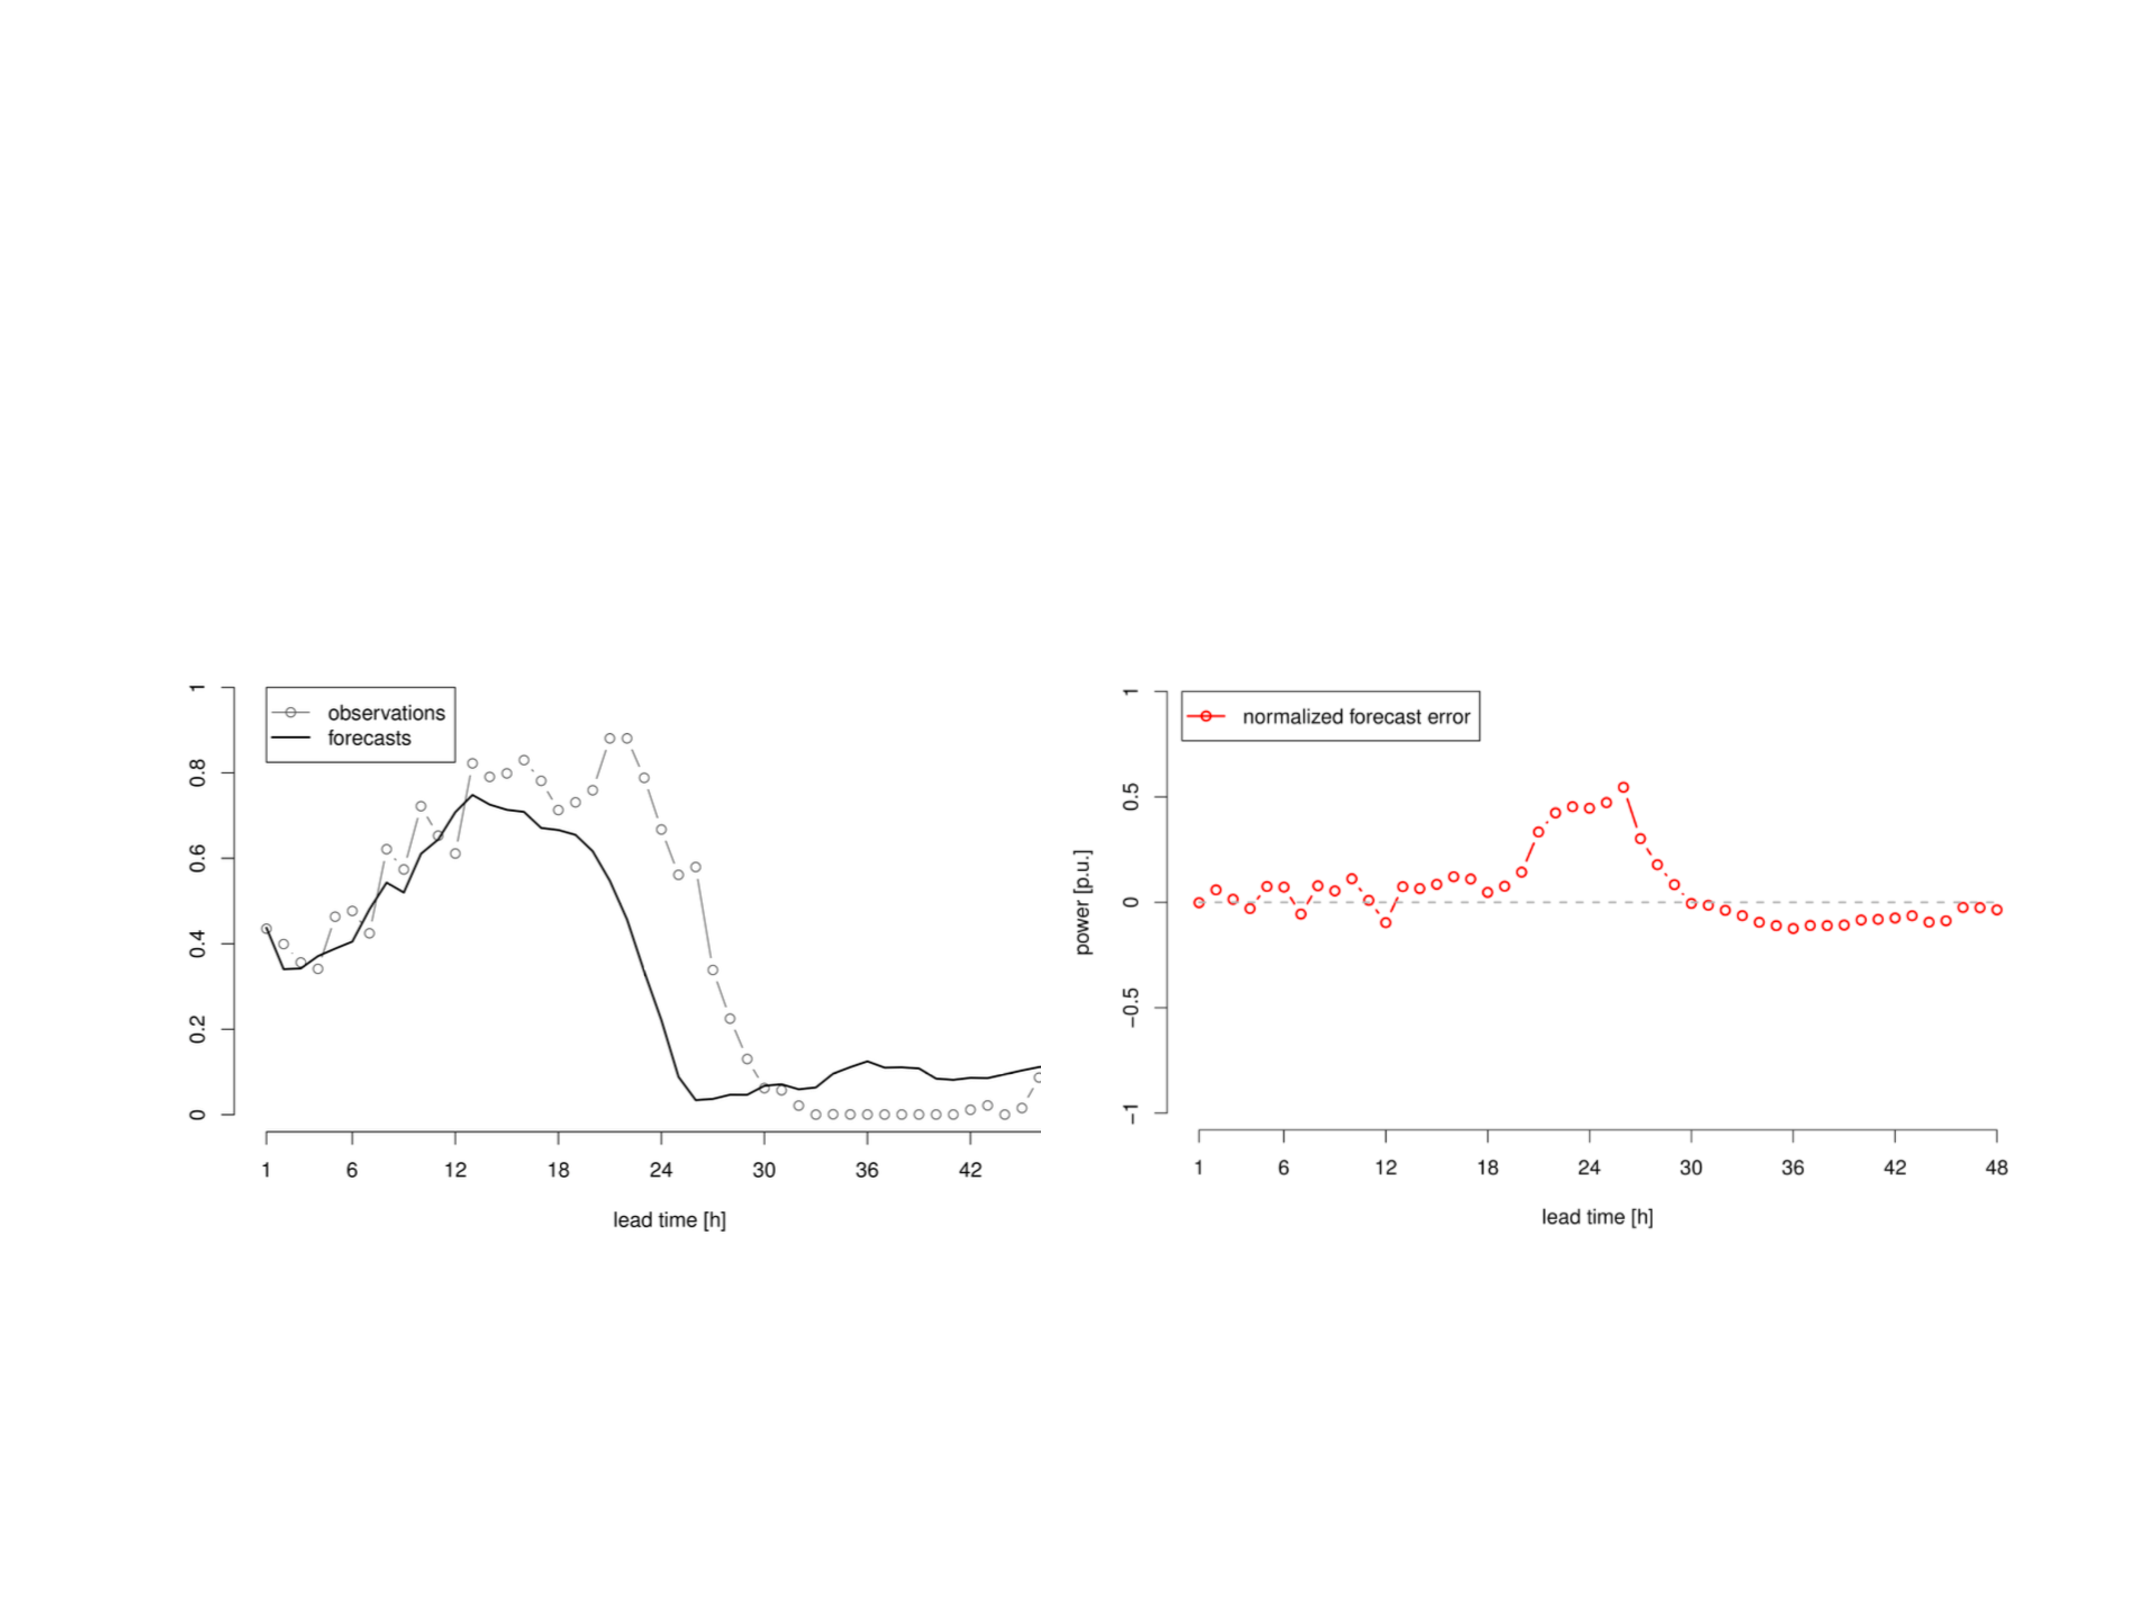
\includegraphics[width=\textwidth]{images/forecast_error_illustration.pdf}
\end{frame}

\begin{frame}{Common error metrics or scores}

\begin{columns}
  \begin{column}{0.45\textwidth}
    Scores are used to summarize aspects of forecast accuracy. 
    
    The most common scores include, \textbf{as a function of the lead time $k$}:
    
    \begin{itemize}
        \item The bias
        $$
        \mathbf{bias}(k)=\frac{1}{T} \sum_{t=1}^T \varepsilon_{t+k \mid t}
        $$
    \end{itemize}
    
  \end{column}
  \begin{column}{0.45\textwidth}
    \begin{itemize}
        \item The Mean Absolute Error (MAE) or NMAE, for the normalized version:
        $$
        \mathbf{MAE}(k)=\frac{1}{T} \sum_{t=1}^T\left|\varepsilon_{t+k \mid t}\right|
        $$
        \item The Root Mean Squared Error (RMSE) or NRMSE, for the normalized version:
        $$
        \mathbf{RMSE}(k)=\sqrt{\frac{1}{T} \sum_{t=1}^T \varepsilon_{t+k \mid t}^2}
        $$
    \end{itemize}    
  \end{column}
\end{columns}
\end{frame}

\begin{frame}{Comparison of three models}
    \begin{center}
        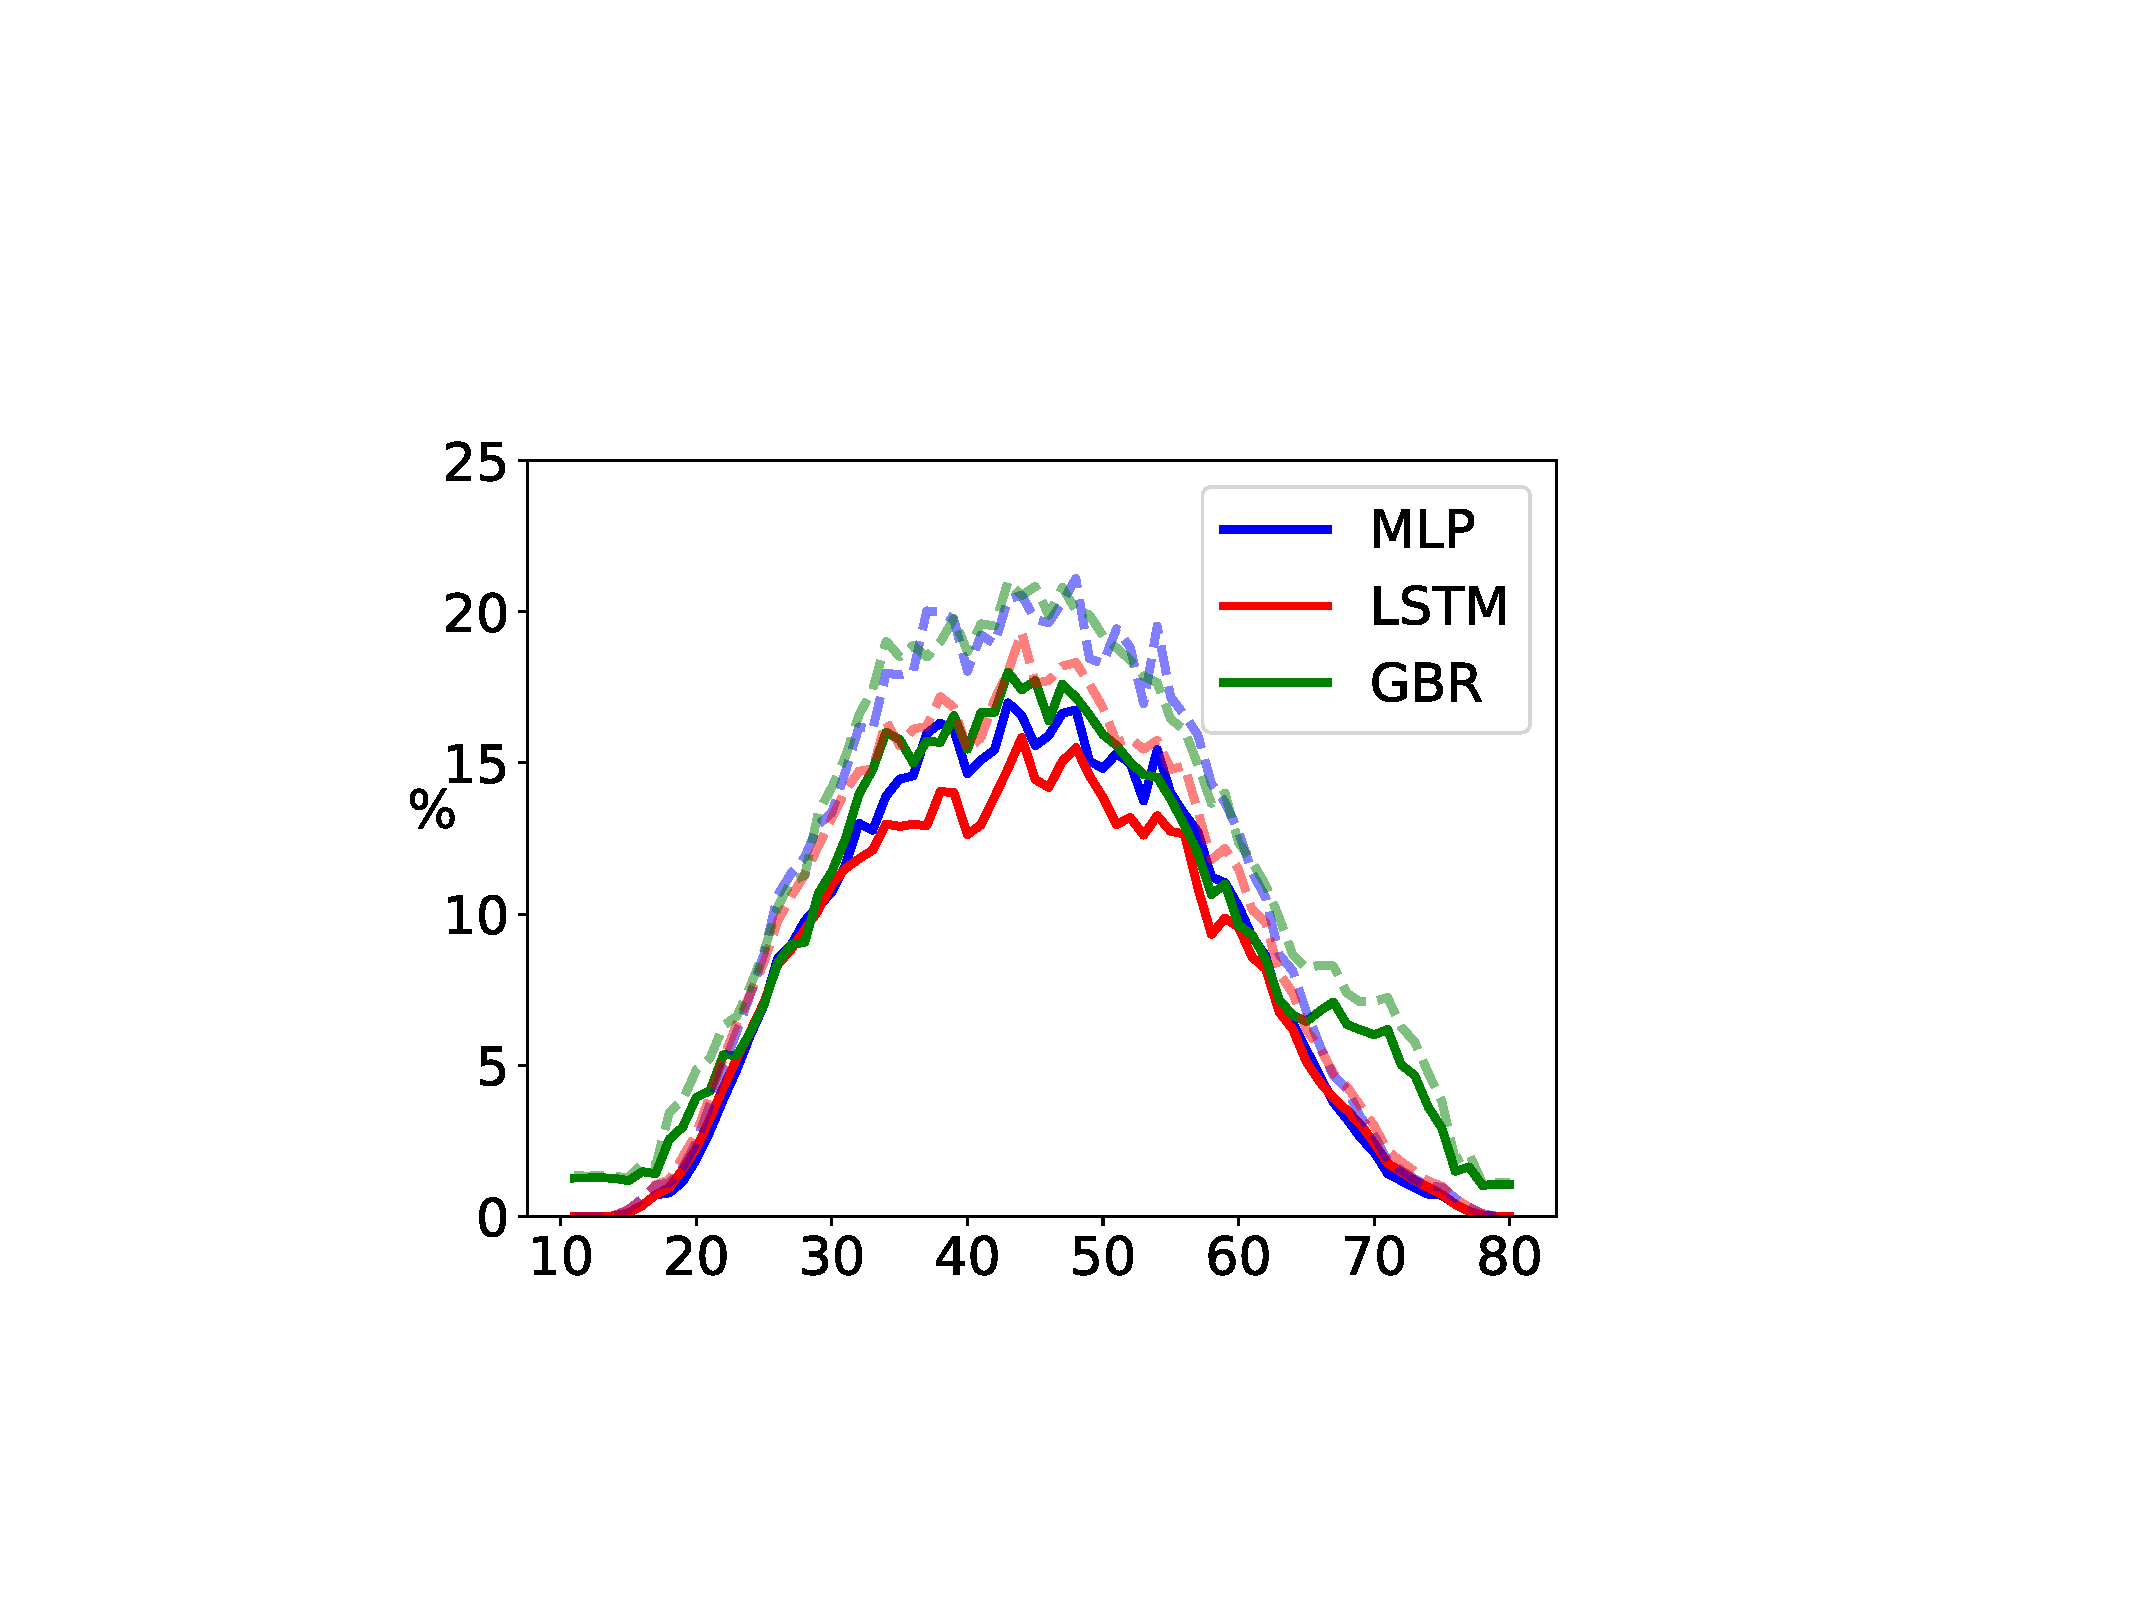
\includegraphics[width=0.6\textwidth]{images/comp_errors_three_models.pdf}\\
        NMAE (plain) and NRMSE (dashed) for three forecasting models.
    \end{center}

\end{frame}

\begin{frame}{Procedure}    
\begin{tikzpicture}[
    % Define the style for the boxes
    block/.style={
        rectangle, 
        draw, 
        text width=7em, 
        text centered, 
        rounded corners, 
        minimum height=5em
        },
        % Define the style for the arrows
        line/.style={
            draw, 
            -Latex, 
            thick
            }
            ]
            % Place the nodes (boxes)
            \node [block] (box1) {Select Data};
            \node [block, right=1cm of box1] (box2) {Select Forecasting methods};
            \node [block, right=1cm of box2] (box3) {Run experimental protocol and fit model};
            \node [block, right=1cm of box3, fill=orange!20] (box4) {Deploy};
            
            % Draw the arrows
            \path [line] (box1) -- (box2);
            \path [line] (box2) -- (box3);
            \path [line] (box3) -- (box4);
            
\end{tikzpicture}
\end{frame}
\subsection{Deployment}
\begin{frame}{Deploy your model}
    \begin{itemize}
        \item Write the data harvesting scripts
        \item Store data in a structured manner
        \item Use visualization tools (e.g. Grafana)
        \item Store your forecasts in a structured manner (do not overwrite them)
        \item Monitor error metrics
    \end{itemize}
\end{frame} 

% Section 4: Probabilistic Forecasting
\section{Probabilistic Forecasting}
\begin{frame}{Handling Uncertainty}
    A single number is dangerous. We need \textbf{Quantile Regression}.
    \vspace{0.3cm}
    Instead of predicting the mean, we predict the $\tau$-th quantile:
    \begin{itemize}
        \item $q_{0.10}$: 10\% chance the actual value is below this (Lower bound).
        \item $q_{0.50}$: The Median.
        \item $q_{0.90}$: 90\% chance the actual value is below this (Upper bound).
    \end{itemize}
    \vspace{0.3cm}
    \textbf{Techniques:} Pinball Loss optimization, Gaussian Processes, or Quantile Regression Forests.
\end{frame}

\begin{frame}{Evaluating Uncertainty: Calibration vs. Sharpness}
    \begin{block}{Calibration (Reliability)}
        Do your 90\% intervals actually contain 90\% of the data?
    \end{block}
    \begin{block}{Sharpness}
        Is the interval narrow enough to be useful for decision-making?
    \end{block}
    \textbf{The Scoring Rule:} \textit{Continuous Ranked Probability Score (CRPS)}
    \[ CRPS(F, y) = \int_{-\infty}^{\infty} (F(x) - \mathbb{1}\{x \geq y\})^2 dx \]
\end{frame}